\documentclass[a4paper]{article}
\usepackage[utf8]{inputenc}
\usepackage{geometry}
\usepackage{amsmath}
\pdfpagewidth
\paperwidth
\pdfpageheight
\paperheight
\usepackage{booktabs}
\usepackage{graphicx}
\usepackage{subfig}
\usepackage{verbatim}
\newcommand*{\unit}[1]{\ensuremath{\mathrm{\,#1}}}
\usepackage{amsthm}
\usepackage{epsfig}
\usepackage{fancyhdr} 
\usepackage{amsmath,amssymb}
\usepackage{amscd} 
\usepackage[T1]{fontenc} 
\usepackage[utf8]{inputenc} 
\usepackage[usenames,dvipsnames]{xcolor}
\usepackage{graphicx,color,listings}
\usepackage{hologo}
\frenchspacing 
\usepackage{float}
\usepackage{geometry}
\usepackage{rotating}
\usepackage{caption}
\captionsetup{labelformat=empty, textfont=sl}
\usepackage{placeins}
\usepackage{hyperref}
\frenchspacing
\title{Esperienza Laboratorio di Fisica Medica: Rivelatori a semiconduttore (Si)}
\author{Simone Lossano, Lorenzo Marini, Jake Harold Pensavalle}
\begin{document}
	\maketitle
	\tableofcontents
	\newpage
	\section{Obiettivi}
L’obiettivo dell’esperienza è descrivere le caratteristiche di un rivelatore a semiconduttore (Silicio)in spettroscopia $\Gamma$. Analizziamo le proprietà del sistema in diverse circostanze e sottoponendolo a diverse sorgenti di radiazione. L'esperienza è divisa in due parti in cui il setup per l'analisi viene cambiato.
	\section{Strumentazione}
Il sistema di analisi è costituito da diversi strumenti collegati tra loro:
\begin{itemize}
\item rivelatore a semiconduttore (diodo al Silicio);
\item generatore di impulsi, che utilizzeremo nella prima fase per produrre impulsi da inviare al
preamplificatore che simulano la risposta del rivelatore;
\item preamplificatore, con capacità intrinseca di \emph{1pF};
\item attenuatori, collegati al preamplificatore, per attenuare con accuratezza il segnale test;
\item amplificatore;
\item oscilloscopio;
\item scheda digitale multicanale;
\item computer;
\item sorgenti radiattive di 241-Am (\emph{Americio}) e 109-Cd(\emph{Cadmio});
\item diversi spessori di rame da \emph{600 $\mu m$};
\item spessori di elementi diversi (Molibdeno, Gadolinio, Stagno, Nickel).
\item un discriminatore contatore di impulsi;

\end{itemize}	
	\section{Calibrazione segnali test}
Vogliamo anzitutto generare dei segnali per simulare lo spettro delle sorgenti radioattive che andremo ad analizzare, così da poter calibrare gli strumenti per le successive acquisizioni con rivelatore. Vengono così creati impulsi tramite il generatore di onde ed osservati attraverso un oscilloscopio multicanale. Infine, lo spettro simulato viene acquisito ed analizzato con un software ("\textbf{MAESTRO}") tramite una DC collegata all'oscilloscopio.  Tramite degli attenuatori modifichiamo le ampiezze dei segnali test, ottenendo le misure riportate nella tabella seguente, al fine di ottenere una calibrazione dell'oscilloscopio multicanale. Vogliamo cos\'i poter stimare i canali corrispondenti alle energie dei fotopicchi dell'Am-241 e del Cd-109 (60 keV, 22 keV). 
	\newline
	
	Come zero della scala del multicanale si imposta il \textbf{channel (Chn) 11}. I segnali test vengono inviati ad un condensatore test da C $\simeq$ 1 pF (in Si $E_{e-h}$ = 3.6 eV). Il tempo di acquisizione è di \textbf{120s}. Riportiamo a titolo d'esempio lo spettro del segnale simulato alla tensione di \emph{4.16 mV} e il relativo fit gaussiano del picco.

\begin{figure}[H]
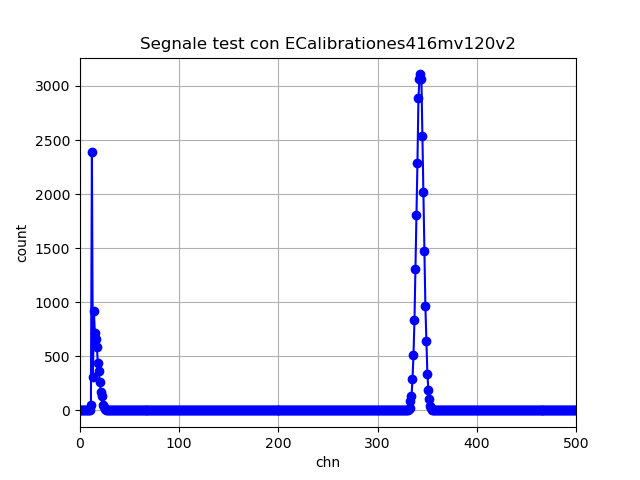
\includegraphics[width=1\textwidth]{Visualecon_ECalibrationes416mv120v2}
        \caption{Fig. 1: Spettro ottenuto tramite il segnale simulato a 4.16 mV.  }
        \label{fig:1}
\end{figure}

\begin{figure}[H]
\includegraphics[width=1\textwidth]{fit_gaussiano_con_ECalibrationes416mv120v2}
        \caption{Fig. 2: Fit Gaussiano ottenuto tramite il segnale simulato a 4.16 mV.  }
        \label{fig:2}
\end{figure}
	
	
\begin{center} 
		
		\begin{tabular}{lcccccc}
			\hline
			\hline
			\textbf{ $\Delta$V} [mV]   &   \textbf{Attenuation} [Db]  	& \textbf{Energy} [KeV]  &  \textbf{Chn}  &   \textbf{FWHM} & \textbf{$\Delta E/E$}\\
			\hline
			\hline
				      $1.04\pm0.01  $    & 43	(30+12+1)  &     $23.40\pm0.23$		        &   $85.59\pm0.02$	&	$8.32\pm0.06  $ & $0.096\pm0.001$	\\
				     $  2.16 1pm0.01$                  &  38 (30+6+2) &         $48.6\pm0.23$   			&	$186.70\pm0.03$  &	$8.19\pm0.04$ &  $0.043\pm0.001$  \\
				       $3.68	\pm0.01  $ 	        &  33.5 (30+2+1+0.5) &        $82.8	\pm0.20$		    & 	$305.38\pm0.03$  &   $8.10\pm0.03$     & $0.026\pm0.001$   \\
				       $4.16	\pm0.001$ 	        & 32.5 (30+2+0.5) &        	  $93.6\pm0.22		$        & 	$342.86\pm0.05$ 	& 	$8.19\pm0.03 $    & $0.023\pm0.01 $ \\
			
			\hline
			\hline
		\end{tabular}
		\linebreak
		\emph{Tab.1: Dati di calibrazione ottenuti tramite fit gaussiano dei picchi.} 
	\end{center}

Tramite la relazione:

     \begin{equation}
     E(\Delta V) = {{C\Delta V}\over{e}} E_{e-h} 
     \end{equation}

abbiamo ricavato i valori di energia, inseriti nella tabella 1, al variare della tensione dei segnali in ingresso per poter ottenere la calibrazione Chn - Energy. 
Una volta ricavati i valori delle energie, sono stati plottati in funzione dei valori dei canali corrispondenti, procedendo con un fit per verificare la linearit\'a (Fig. 3). Lo stesso viene fatto per verificare quindi la linearità della relazione Tensione-Chn.
\newpage

\begin{figure}[H]
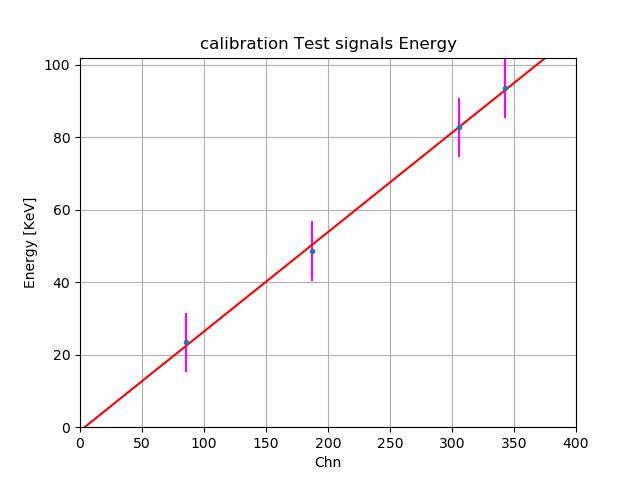
\includegraphics[width=1\textwidth]{calibration_test_signals_energy}
        \caption{Fig. 3: Fit per la calibrazione dei segnali di test. I parametri stimati sono il coefficiente angolare $m$ = 0.274 $\pm$ 0.007, e l'intercetta \'e 1.930 $\pm$ 1.658}
        \label{fig:3}
\end{figure}

\begin{figure}[H]
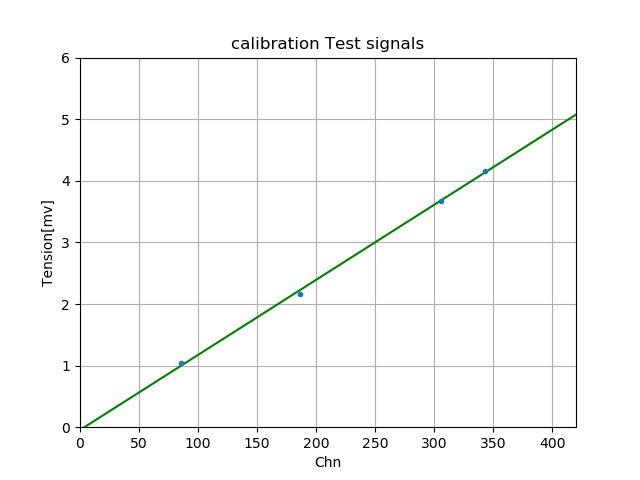
\includegraphics[width=1\textwidth]{calibration_test_signals}
        \caption{Fig. 4: Fit lineare Tensione-Channel. I parametri stimati sono il coefficiente angolare $m$ = 0.012 $\pm$ 0.005, e l'intercetta \'e 0.089 $\pm$ 0.072.}
        \label{fig:4}
\end{figure}

Dal fit otteniamo quindi la relazione:
\begin{equation}
f(x)_{fit}=(0.221 \pm 0.122)x + (2.162 \pm 30.653)
\end{equation}

Invertendo la relazione, ricaviamo i valori attesi per i canali per i fotopicchi a 59.6 keV e 22.6 keV: \textbf{Chn(59.6keV) = 257.8}, \textbf{Chn(22.6keV) = 92.5}.
\newpage

Trovato il miglior setting dei parametri, studiamo come varia la risoluzione energetica in funzione dell'attenuazione del segnale (Gain). Tali valori sono ricavati a partire da quelli in Tabella 1. 

\begin{figure}[H]
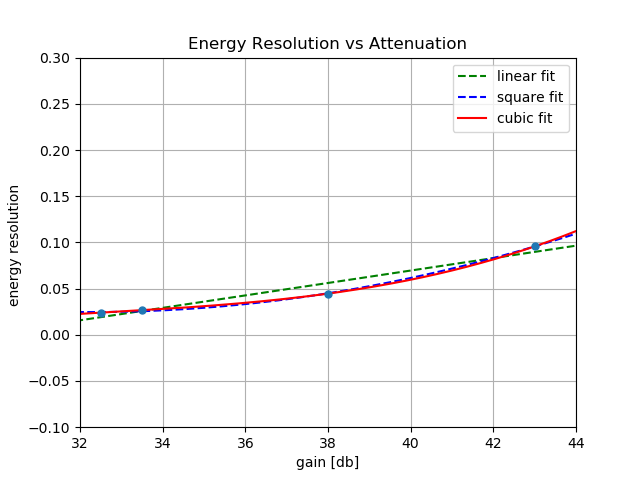
\includegraphics[width=1\textwidth]{resvsgain}
        \caption{Fig. 5: Fit per l'energia in funzione dell'attenuazione (gain) dell'ampiezza del segnale. Un'interpolazione di dati mostra come questi siano meglio fittati da una funzione cubica (valore di $R^2$ più vicino ad 1) del tipo $ax^3+bx^2+cx+d$, con $a=0.0004 $, $b=0.05194 $, $c=-1,8664 $, $d=22.2016 $ ed $R^2=0.999$}.
        \label{fig:5}
\end{figure}

\newpage

\section{Risoluzione energetica in funzione delle capacit\'a e valutazione del rumore del sistema}

Trovato il giusto setting dei parametri, abbiamo collegato al preamplificatore diversi cavetti LEMO (che serviranno a collegare il rivelatore al setup) che costituiscono delle capacit\'a. Utilizziamo un segnale di ampiezza \textbf{4.16 mV} (Tab.1) e lo testiamo per diversi valori 

\begin{center} 
		
		\begin{tabular}{lcccc}
			\hline
			\hline
			\textbf{Capacity} [pF]   &     \textbf{FWHM}         	&  \textbf{Chn}              &     \textbf{Net Area}    	 \\
			\hline
			\hline
				       6.9                      & $8.50\pm0.06$  			&       344.20$\pm$0.02			        	&	27714 $\pm$ 166						\\
				       27.1                   &  9.94 $\pm$0.07			&        344.64  $\pm$0.03  				  	&	27666 $\pm$ 166			  			\\
				       18.6		        &  9.09 $\pm$0.05				&       345.49  $\pm$0.02 			             & 	27699 $\pm$ 166			 			\\
				       12.4		        & 8.76 	$\pm$0.05		&        342.62  $\pm$0.03  			       	& 	27690 $\pm$ 166						\\
			    		?			& 8.78	$\pm$0.04		&	  346.18	$\pm$0.03		      	&	27697 $\pm$ 166							\\
			\hline
			\hline
		\end{tabular}
		\linebreak
		\emph{Tab.2: Dati ottenuti tramite il fit gaussiano dei picchi osservati al variare della capacità. Le energie sono state trovate tramite la funzione di calibrazione trovata precedentemente. Con "?" è indicata la capacità incognita.} 
	\end{center}
	
\begin{center} 
		
		\begin{tabular}{lcc}
			\hline
			\hline
			\textbf{Capacity} [pF]   &     \textbf{$\Delta E/E$} 	 \\
			\hline
			\hline
				       6.9              &	0.025 +- 0.001 \\
				       27.1             &	0.029 +- 0.001  \\
				       18.6		        &	0.026 +- 0.002 \\
				       12.4		        & 	0.025 +- 0.002  \\
			    		?			    &  	0.025 +- 0.002 \\
			\hline
			\hline
		\end{tabular}
		\linebreak
		\emph{Tab.3: Capacità vs risoluzione energetica, quest'ultima ottenuta utilizzando le energie dei picchi in Tabella 1} 
	\end{center} 	
	
L'interpolazione dei dati mostra come questi ultimi siano meglio fittati tramite una funzione quadratica.

\begin{figure}[H]
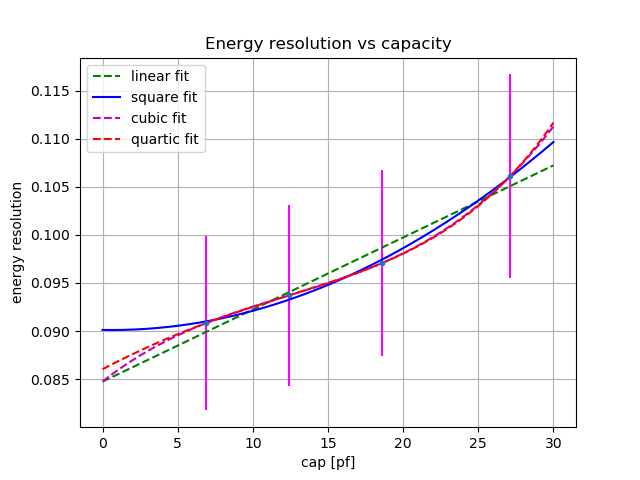
\includegraphics[width=1\textwidth]{resvvscapacity}
        \caption{Fig. 6: Fit per la risoluzione energetica in funzione della capacità. I punti sono meglio interpolati tramite una funzione del tipo $ax^4+bx^3+cx^2+dx+e$. I valori stimati dei coefficienti sono: $a = 0.0000005$, $b = -0.000012$, $c = -0.00031$, $d=0.010$, $e=0.042$ con $R^2 = 0.999$.}
        \label{fig:6}
\end{figure}

\newpage

Dal fit possiamo così stimare il valore della capacità incognita tramite la risoluzione energetica, che risulta essere pari a \textbf{13.6$\pm0.1$ pF}.


Per quanto riguarda la valutazione del rumore introdotto dalla capacità sul segnale, sappiamo che:

     \begin{equation}
     FWHM_{tot}^2=FWHM_{stat}^2+FWHM_{noise}^2+FWHM_{drift}^2
     \end{equation}
     
Avendo eseguito nuovamente le misure dopo un ragionevole intervallo di tempo, notiamo dal programma MAESTRO che non ci sono cambiamenti apprezzabili della posizione del picco, per cui possiamo supporre la componente di \emph{drift} del rumore $\simeq 0$.
Avendo utilizzato sempre lo stesso segnale in ingresso, possiamo supporre che la $FWHM_{stat}^2$ sia costante (1,73), quindi, avendo precedentemente analizzato l'andamento della risoluzione energetica in funzione della capacità, possiamo supporre inoltre che la $\sigma_{noise}$ presenti circa lo stesso andamento in funzione della capacità, a meno di una costante additiva. Infatti, ogni altra componente alla risoluzione oltre la $FWHM_{noise}$ per i punti in Fig.6, rimane la stessa.

\section{Studio dello spettro di sorgenti radioattive $\gamma$.}
Abbiamo due tipi di sorgenti radioattive a disposizione: \textbf{241-Am} e \textbf{109-Cd}. 

\subsection{Americio}
Anzitutto colleghiamo il rivelatore (quello fornitoci è contrassegnato come \textbf{n.o 4}) al preamplificatore, scolleghiamo il generatore d'onde e, successivamente, procediamo a piazzare dentro un apposito foro nel rivelatore la sorgente di \textit{241-Am}.  Trattandosi di una giunzione p-n, cerchiamo il valore ottimale di tensione da fornire allo strumento affinchè sia in regime di sovrasvuotamento. 
\\

Facciamo una prima acquisizione dello spettro con una tensione di 4.0 V, notiamo che in corrispondenza del supposto picco a 59.6 KeV se ne presentano invece due ravvicinati (Fig. 4, sotto). Il motivo sembra essere che il valore della tensione scelto non sia sufficiente affinchè la larghezza della zona di svuotamento sia tale da far sì che l'intera carica di ionizzazione prodotta dai fotoni emessi dalla sorgente venga raccolta.

\begin{figure}[H]
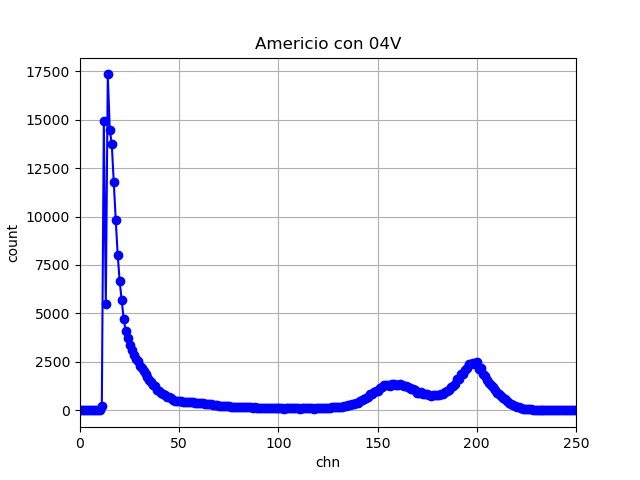
\includegraphics[width=1\textwidth]{Americio_con_04V}
        \caption{Fig. 7: Spettro dell'Americio con tensione 4.0V. Si notano due picchi ravvicinati in corrispondenza della zona dove ci                                     						 aspetteremmo il fotopicco a causa del valore di tensione di svuotamento troppo basso.}
        \label{fig:7}
\end{figure}

Viene quindi osservato il fotopicco dell'Americio per diversi valori di tensione (riportati in Tab.4) per cercare quella di lavoro (cioè una in cui ci sia sovrasvuotamento della regione di carica spaziale).
Abbiamo proceduto nell'analizzare i picchi con un fit gaussiano dei dati ottenendo i risultati in tabella.

\begin{figure}[H]
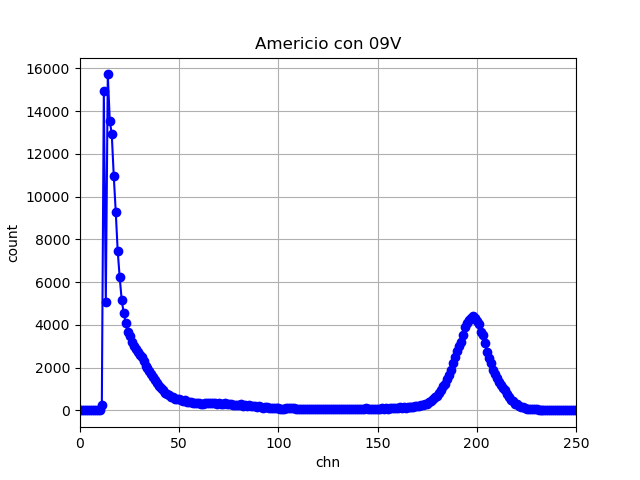
\includegraphics[width=01\textwidth]{Americio_con_09V}
        \caption{Fig. 8: Spettro dell'Americio con tensione 9.0V. .}
        \label{fig:8}
\end{figure}

\begin{figure}[H]
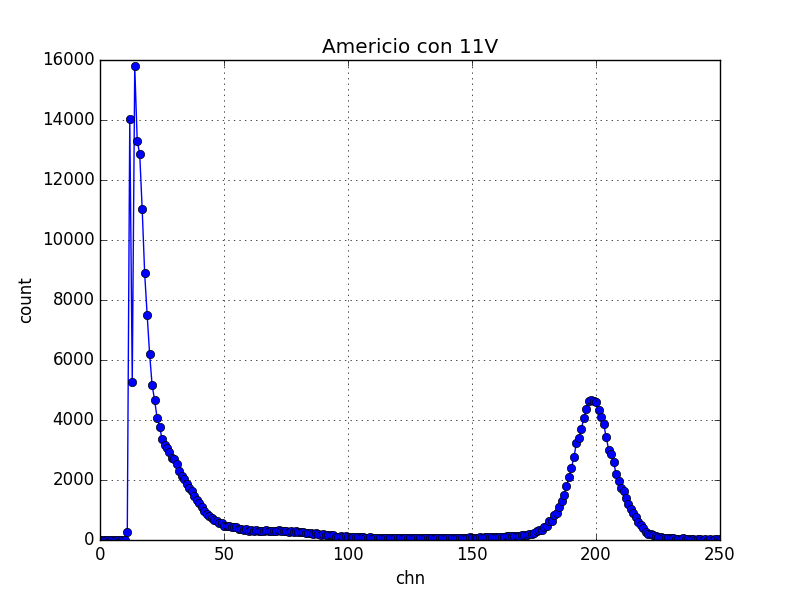
\includegraphics[width=01\textwidth]{Americio_con_11V}
        \caption{Fig. 9: Spettro dell'Americio con tensione 11.0V. .}
        \label{fig:9}
\end{figure}

\begin{figure}[H]

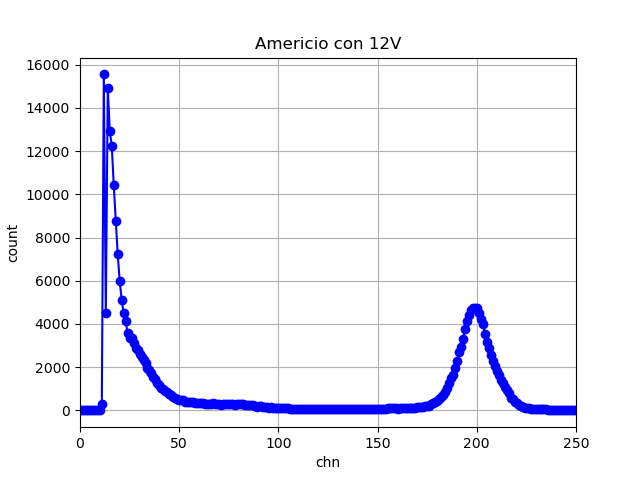
\includegraphics[width=01\textwidth]{Americio_con_12V}
        \caption{Fig. 10: Spettro dell'Americio con tensione 12.0V. .}
        \label{fig:10}
\end{figure}  
\newpage
	
\begin{center} 
		
		\begin{tabular}{lccccc}
			\hline
			\hline
			\textbf{$\Delta V$} [V]   &     \textbf{Chn}		&     \textbf{Energy} [KeV]		&     \textbf{FWHM}		&     \textbf{Net Area} 	& \textbf{Risoluzione energetica} \\
			\hline
			\hline
				       4.0             &	198.94	$\pm0.16$		&		46.12	$\pm$0.30		&				22.85 $\pm$0.39		&			54727 $\pm$ 398 & 0.116 $\pm$0.001\\
				       9.0             &	197.64 $\pm0.09$			&		45.83	$\pm$0.32		&				20.59 $\pm$0.21		&			91390 $\pm$ 399&0.104$\pm$0.001\\
				       11.0		        &	198.97 $\pm$0.10			&		46.13$\pm$0.31			&				19.57 $\pm$0.23		&			92393 $\pm$ 393&0.098$\pm$0.001\\
				       12.0		        & 	198.85$\pm$0.10	 			&		46.10$\pm$0.28			&				19.20$\pm$0.24		&			91896 $\pm$ 397&0.096$\pm$0.001\\
			\hline
			\hline
		\end{tabular}
		\linebreak
		
		\emph{Tab.4: Dati del fotopicco dell'Americio a diverse tensioni di svuotamento del rivelatore. L'energia del picco è 							 stata trovata tramite la funzione di calibrazione ricavata precedentemente.  } 
	\end{center} 	
\'E anzitutto evidente che l'energia ottenuta dalle acquisizioni per il fotopicco dell'Americio non sia quella attesa. Tale discrepanza è possibile ricordando che il rivelatore è dotato di una capacità interna che non conosciamo. 
Possiamo notare però che per valori di tensione intorno ai \emph{12 V}, la posizione del picco e la Net Area sono circa costanti. \'E ragionevole pensare perciò che siamo in condizione di sovrasvuotamento, scegliamo quindi come tensione di lavoro \textbf{12 V}.
\\



\begin{figure}[H]
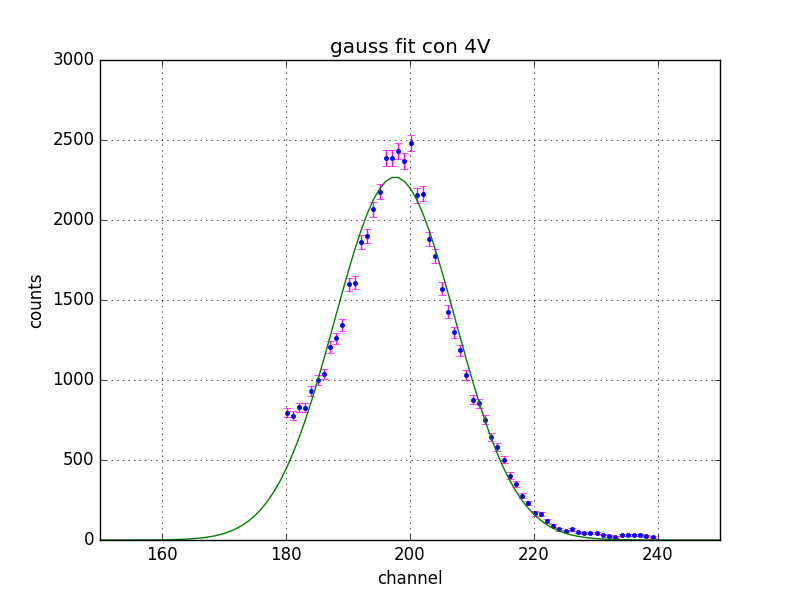
\includegraphics[width=1\textwidth]{Fit_Gaussiano_con_4V}
        \caption{Fig. 11: Fit Gaussiano del picco a 4.0 V. In questo caso viene analizzato solo il picco al Chn 198.}
        \label{fig:11}
  \end{figure}
  
  \begin{figure}[H]
  
  
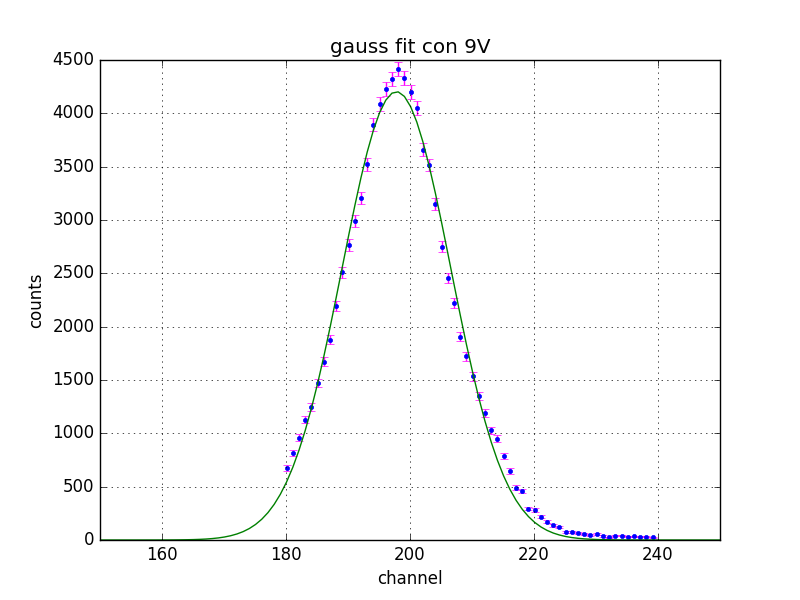
\includegraphics[width=1\textwidth]{Fit_Gaussiano_con_9V}
        \caption{Fig. 12: Fit Gaussiano del picco a 9.0 V}
        \label{fig:12}
\end{figure}

\begin{figure}[H]
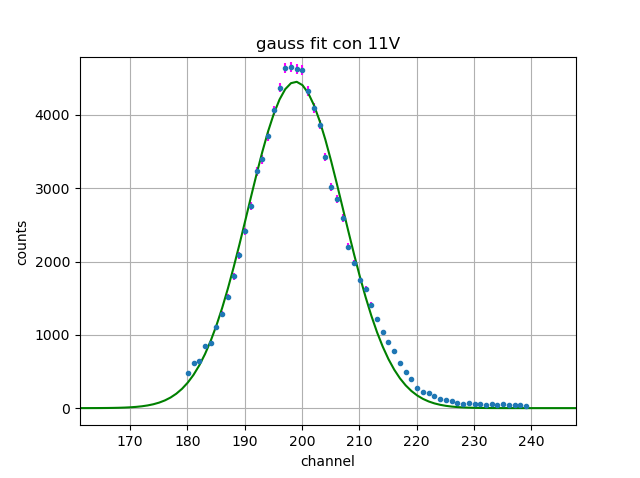
\includegraphics[width=1\textwidth]{Fit_Gaussiano_con_11V}
        \caption{Fig. 13: Fit Gaussiano del picco a 11.0 V}
        \label{fig:13}
        \end{figure}
        
        \begin{figure}[H]
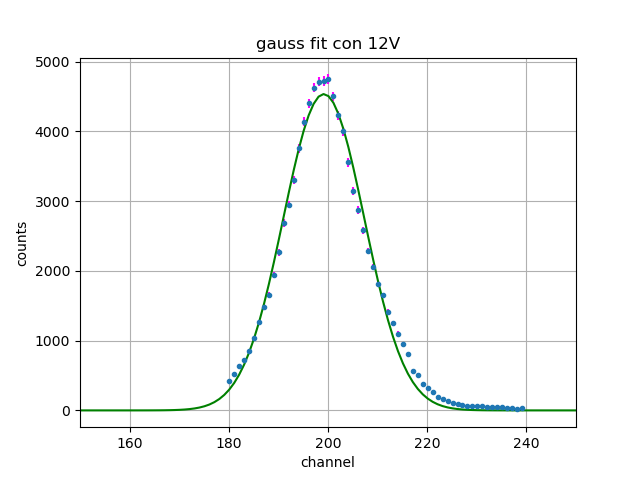
\includegraphics[width=1\textwidth]{Fit_Gaussiano_con_12V}
        \caption{Fig. 14: Fit Gaussiano del picco a 12.0 V}
        \label{fig:14}        
\end{figure}
\newpage


	
Dai dati così ottenuti, plottiamo la FWHM e <x> in funzione della tensione di svuotamento.

\begin{figure}[H]
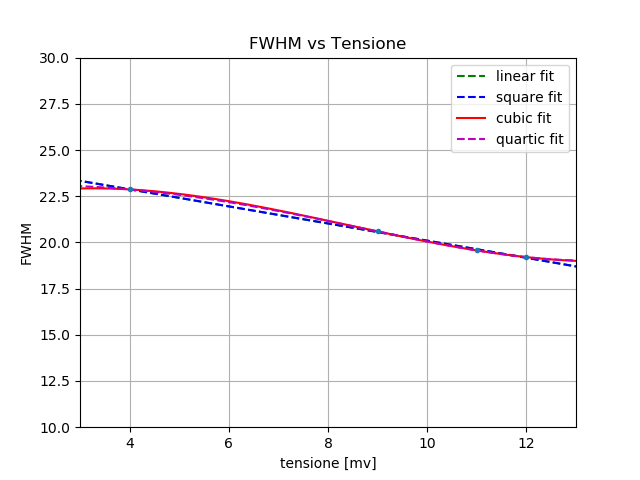
\includegraphics[width=1\textwidth]{FWHM_vs_Tensione}
        \caption{Fig. 15: FWHM in funzione tensione di svuotamento. Si vede che i punti sono meglio fittati tramite una funzione cubica del tipo $ax^3+bx^2+cx+d$, con coefficienti $a=-0.059$, $b=1.407$, $c=-10.136$, $d=219.42$, $R^2= 1.000$.}
        \label{fig:15}
\end{figure}

\begin{figure}[H]
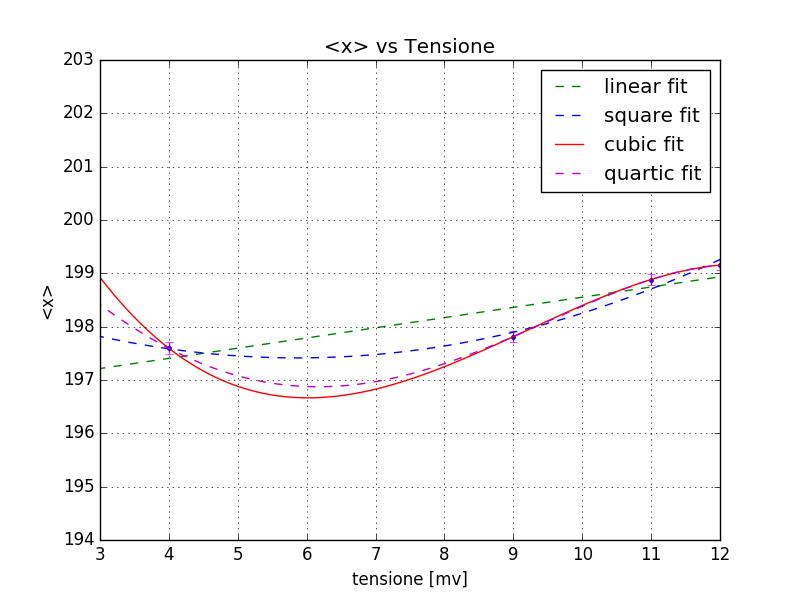
\includegraphics[width=1\textwidth]{x_vs_Tensione}
        \caption{Fig. 16: <x> in funzione della tensione di svuotamento. Si vede che i punti sono meglio fittati tramite una funzione cubica del tipo $ax^3+bx^2+cx+d$, con coefficienti $a=0.057$, $b=-1.298$, $c=8.642$, $d=5.425$, $R^2= 1.000$}
        \label{fig:16}
\end{figure}
\newpage

\subsection{Cadmio}
In letteratura troviamo che il Cadmio presenta tre picchi: a 22.1 KeV, 25 KeV, 88KeV. Lavoriamo sempre alla tensione di svuotamento scelta per il rivelatore, cioè \textbf{12V} e per un tempo di acquisizione di \textbf{900s}. Dallo spettro visualizzato tramite MAESTRO, appare distinguibile un solo picco in corrispondenza del Chn 74, dove supponiamo i primi due picchi si siano sovrapposti, con il secondo che appare come una gobba sul picco a 22.1 KeV. Il picco a 88 KeV è invece assente poichè il tempo di acquisizione è insufficiente per avere una statistica apprezzabile.  
\begin{center} 
		
		\begin{tabular}{lcccc}
			\hline
			\hline
			\textbf{Chn}      &     \textbf{Energy} [KeV]  &     \textbf{FWHM} &     \textbf{Net Area} 	 \\
			\hline
			\hline
				      74.90  &	15.50	&		2.18 		& 2635 $\pm$ 59			\\
				       
			\hline
			\hline
		\end{tabular}
		\linebreak
		\emph{Tab.6: Dati del picco del Cadmio visualizzati tramite MAESTRO.} 
	\end{center} 	
Eseguiamo un fit gaussiano del picco ed otteniamo i seguenti dati:

\begin{center} 
		
		\begin{tabular}{lccccc}
			\hline
			\hline
			\textbf{Chn} & \textbf{$\sigma$}  &     \textbf{Energy} [KeV]  &     \textbf{FWHM}  & \textbf{Risoluzione Energetica}   & \textbf{Net Area} 	 \\
			\hline
			\hline
				       75.13 $\pm$0.03  & 4.58$\pm$0.05          &	20.71 $\pm$0.02	&		10.76 $\pm$ 0.10 & 0.15 $\pm$ 0.03		& 2557 $\pm$ 59			\\
				       
			\hline
			\hline
		\end{tabular}
		\linebreak
		\emph{Tab.7: Dati del picco del Cadmio ottenuti tramite il fit gaussiano.} 
	\end{center}
	
\begin{figure}[H]
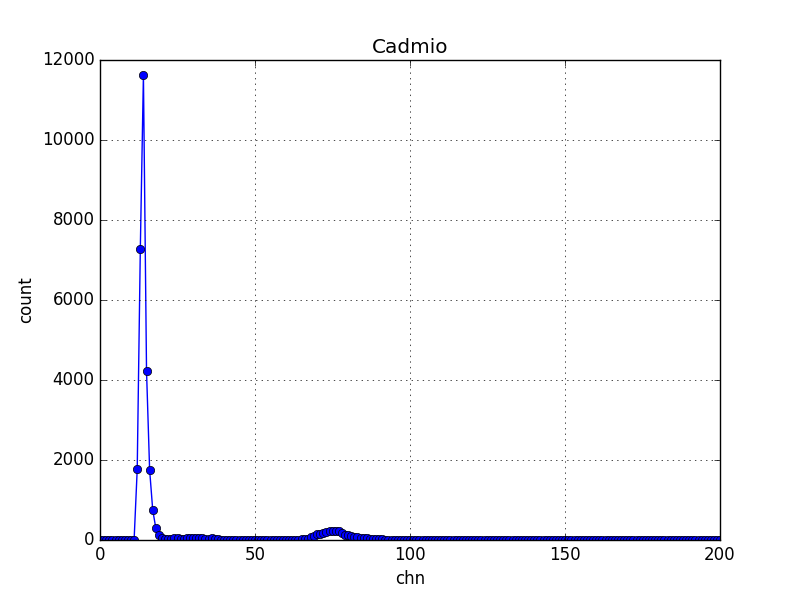
\includegraphics[width=0.8\textwidth]{cadmio.png}
        \caption{Fig. 17: Spettro del Cadmio, tempo di acquisizione 900s.}
        \label{fig:17}
\end{figure}
\begin{figure}[H]
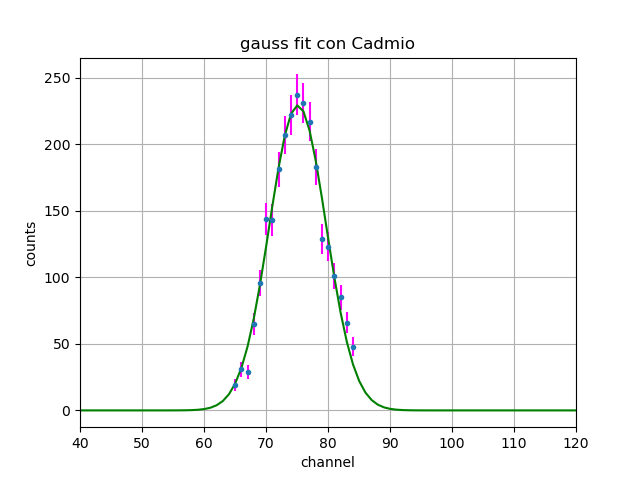
\includegraphics[width=0.8\textwidth]{fit_gaussiano_con_Cadmio.png}
        \caption{Fig. 18: Fit gaussiano del fotopicco del Cadmio.}
        \label{fig:18}
\end{figure}
\subsection{Calibrazione delle sorgenti e studio dello spettro con spessori.}

Dalle misure delle energie dei picchi acquisite dagli spettri dell'Americio e del Cadmio, vogliamo ottenere una nuova calibrazione Energy-Chn. Abbiamo però a disposizione solo due punti, per trovarne altri, che permettano di ottenere un fit, ricerchiamo altri picchi frapponendo tra la sorgente e il rivelatore lamine di vari materiali. Abbiamo a nostra disposizione:
\begin{itemize}
\item Gadolinio, spessore: $120 \mu m$
\item Gadolinio impuro, $100 \mu m$
\item Molibdeno, $50 \mu n$, $100 \mu m$
\item Stagno, $125 \mu m$
\item Nichel, $20 \mu m$
\end{itemize}




In letteratura sono note le energie dei fotoelettroni delle principali linee di emissione delle shell K,L ed M [rif. Radiation Detection and Measurements, G.F. Knoll].
 Ci aspettiamo così di vedere almeno il picco \textbf{$K_{\alpha_{1}}$} che si ottiene frapponendo questi materiali, oltre che il fotopicco, normalmente a 60 KeV, dell'Americio. \\
Lavoriamo sempre con una tensione di 12V sul rivelatore e il tempo d'acquisizione è fissato a \textbf{120 s}. Per ogni spessore vengono quindi osservati i picchi tramite MAESTRO (il fit gaussiano non converge a causa della poca statistica). I risultati sono raccolti nelle Tab. 8,9, in Fig.19 la calibrazione con i picchi ottenuti.\\
\begin{figure}[H]
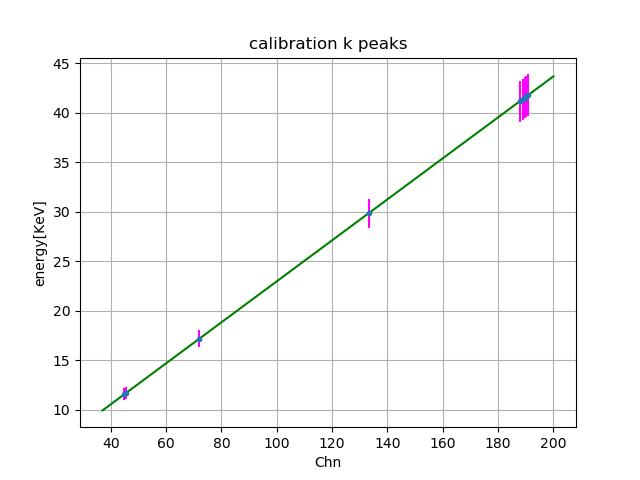
\includegraphics[width=0.8\textwidth]{calibration_test_signals_new}
        \caption{Fig. 19: Fit lineare per la calibrazione delle sorgenti radioattive, tempo di acquisizione 120s.}
        \label{fig:19}
\end{figure}        
\newpage
Dal fit otteniamo i valori per la retta di calibrazione Chn-Energy:
\begin{equation}
f(x)_{fit}=0.21x+2.28
\end{equation}


\begin{center} 
		
		\begin{tabular}{lcccccc}
			\hline
			\hline
			\textbf{Elemento spessore} & \textbf{Chn}  &   \textbf{FWHM} & \textbf{Energy} [KeV] & \textbf{$Energy_{rif}$} [KeV]  & \textbf{Net Area}	\\
			\hline
			\hline
				      Sn(125$\mu m$) &  82.95   & 2.50 & 19.69	& 25.27 & 6182	$\pm$	162	\\
				      Mo(100$\mu m$) &  56.53   & 1.75 	& 14.15 & 17.48 & 1107	$\pm$	124 \\
				      Mo(50$\mu m$) &  55.93	& 1.67	& 14.02	& 17.48 & 1318		$\pm$	199 \\
				      Gd(120$\mu m$) &  144.18	& 2.06 	& 32.55	& 42.99 & 1443	$\pm$	107 \\
				      Gd (100$\mu m$,ossidato) &  144.50 & 1.92 & 42.99 & 32.63	&  1547	$\pm$	99 \\
				      
			\hline
			\hline
		\end{tabular}
		\linebreak
		\emph{Tab.8: Dati ottenuti tramite MAESTRO dei picchi $K_{\alpha_{1}}$, visualizzati a sinistra rispetto al fotopicco dell'americio nello spettro. Le energie sono state calcolate invece tenendo conto della funzione di calibrazione. $E_{rif}$ sono le energie dei picchi $K_{\alpha_{1}}$ riportate in letteratura.} 
	\end{center}
Notiamo delle discrepanze con i valori in letteratura, questo, come già detto precedentemente, potrebbe in parte essere dovuto alla capacità incognita all'interno del rivelatore.	

\begin{center} 
		
		\begin{tabular}{lccccc}
			\hline
			\hline
			\textbf{Elemento spessore} & \textbf{<x>}  &   \textbf{$\sigma$} &\textbf{FWHM}  & \textbf{Net Area}	\\
			\hline
			\hline
				      Sn(125$\mu m$) &  201.39$\pm$0.03   & 5.50$\pm$0.06  & 12.92$\pm$0.10   &  59351	$\pm$	215	\\
				      Mo(100$\mu m$) &  200.27$\pm$0.03   & 6.28$\pm$0.07 & 14.75$\pm$0.12	&  74515	$\pm$	142 \\
				      Mo(50$\mu m$) &  200.09$\pm$0.04	& 7.05	$\pm$0.08 & 16.56$\pm$0.14 &  87285		$\pm$	111 \\
				      Gd(120$\mu m$) &  202.03$\pm$0.03	& 4.99$\pm$0.07	 & 11.72$\pm$0.09  &  41956	$\pm$	67 \\
				      Gd (100$\mu m$,ossidato) &  201.68$\pm$0.03& 5.33$\pm$0.06 & 12.52$\pm$0.10	&  50862	$\pm$	47 \\
				      
			\hline
			\hline
		\end{tabular}
		\linebreak
		\emph{Tab.9: Dati ottenuti tramite fit gaussiano del fotopicco dell'Americio per diversi spessori.} 
\end{center}

\subsection{Attenuazione in un materiale}
Vogliamo valutare la legge di attenuazione in un materiale:
\begin{equation}
I=I_{0}e^{-\mu x}
\end{equation}
Utilizzeremo degli spessori di rame da \textbf{600 $\mu m$}, posizionati in modo da formare uno spessore crescente tra la sorgente di Americio e il rivelatore con tempi di acquisizione di \textbf{60 s}. Viene preventivamente fatta un'acquisizione della sola sorgente per valutare eventuali cambiamenti rispetto alle misure iniziali, non si osservano sostanziali variazioni.\\

Riportiamo i valori dei picchi osservati tramite MAESTRO e successivamente quelli ottenuti dal fit gaussiano.

\begin{center} 
		
		\begin{tabular}{lcccc}
			\hline
			\hline
			\textbf{N.o spessori} & \textbf{Chn}  &   \textbf{FWHM}   & \textbf{Net Area}	\\
			\hline
			\hline
				      1 &  201.36   & 2.38  &  27259	$\pm$	215	\\
				      2 &  202.24   & 2.20	&  14953	$\pm$	142 \\
				      3 &  202.74	& 2.09	&  7842		$\pm$	111 \\
				      4 &  202.88	& 1.83	&  3967	$\pm$	67 \\
				      5 &  203.17	& 1.94	&  1889	$\pm$	47 \\
				      6 &  202.62	& 1.88	&  904	$\pm$	33 \\
				      7 &  203.10	& 1.15	&  446	$\pm$	24 \\
				      8 &  202.23	& 1.03	&  236	$\pm$	16 \\
				      9 &  200.17	& 0.26	&  124	$\pm$	12 \\
				      10 & 204.23	& 0.83	&  66	$\pm$	8 \\
			\hline
			\hline
		\end{tabular}
		\linebreak
		\emph{Tab.10: Dati ottenuti tramite MAESTRO del picco dell'Americio a diversi spessori di Cu.} 
\end{center}
 Riportiamo di seguito a titolo esemplificativo alcuni grafici estratti dall'analisi dati.
 

\begin{figure}[H]
	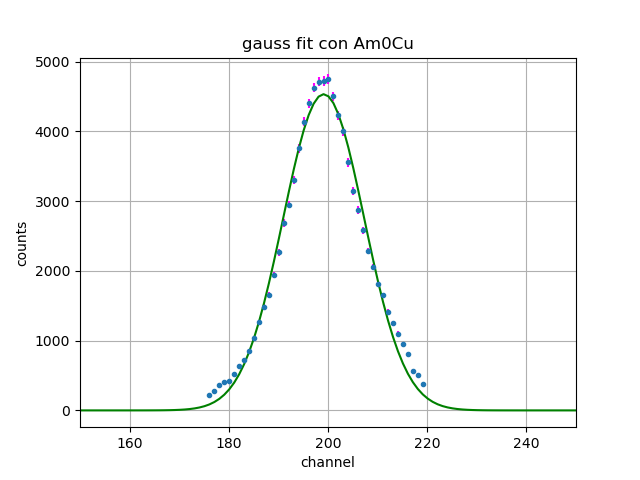
\includegraphics[width=1\textwidth]{gauss_fit_con_Am0Cutext}
        \caption{Fig. 20: Fit Gaussiano del picco senza spessori.}
        \end{figure}
        \label{fig:20} 
        \begin{figure}
        
            
	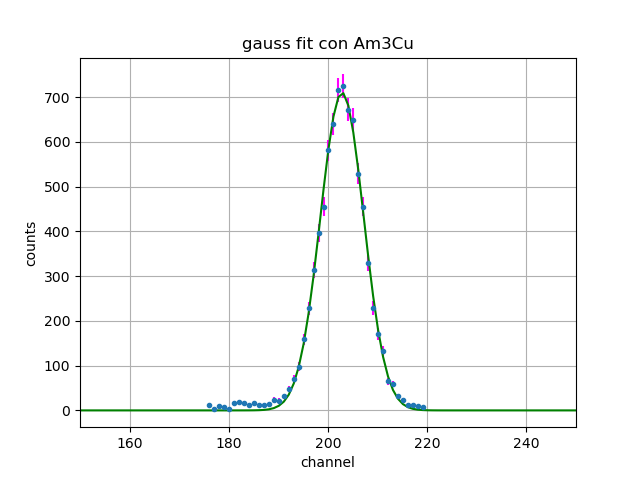
\includegraphics[width=1\textwidth]{gauss_fit_con_Am3Cutext}
        \caption{Fig. 21: Fit Gaussiano del picco con 3 spessori}
        \label{fig:21}
        

\end{figure}

\begin{figure}[H]
	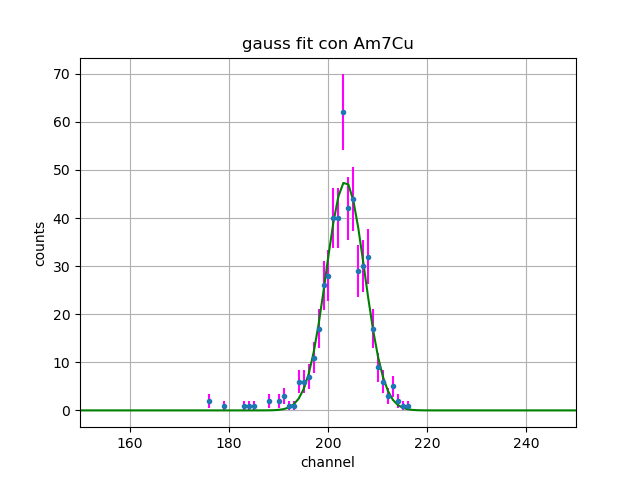
\includegraphics[width=1\textwidth]{gauss_fit_con_Am7Cutext}
        \caption{Fig. 22: Fit Gaussiano del picco con 7 spessori}
        \label{fig:22}
	\end{figure} 
	\begin{figure}
	
	
	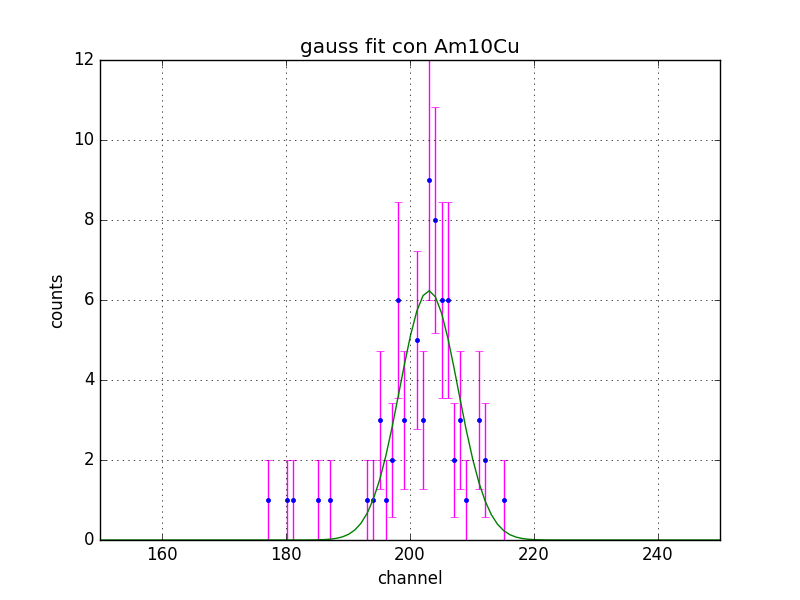
\includegraphics[width=1\textwidth]{gauss_fit_con_Am10Cutext}
        \caption{Fig. 23: Fit Gaussiano del picco con 10 spessori}
        \label{fig:23}        
\end{figure}  


\newpage

In Tab.11 i valori ottenuti tramite fit gaussiano:

 
\begin{table}[H]
	
		\begin{tabular}{lccccc}
			\hline
			\hline
			\textbf{N.o spessori} & \textbf{<x>}  &   \textbf{$\sigma$} &\textbf{FWHM}   & \textbf{Net Area}	\\
			\hline
			\hline
				      1 &  201.46$\pm$0.40   & 5.38$\pm$0.07 &  12.64$\pm$0.12 &  27259	$\pm$	215	\\
				      2 &  202.38 $\pm$0.33  & 4.68$\pm$0.05 & 11.00$\pm$0.10	&  14953	$\pm$	142 \\
				      3 &  202.83$\pm$0.26	& 4.38$\pm$0.04 & 10.29$\pm$0.10	&  7842		$\pm$	111 \\
				      4 &  202.97$\pm$0.42	& 4.11$\pm$0.04 & 9.65$\pm$0.09	&  3967	$\pm$	67 \\
				      5 &  203.16$\pm$0.33	& 4.19$\pm$0.04 & 9.84$\pm$0.10	&  1889	$\pm$	47 \\
				      6 &  202.81$\pm$0.44	& 4.39$\pm$0.05 & 10.31$\pm$0.11	&  904	$\pm$	33 \\
				      7 &  203.51$\pm$0.37	& 3.86$\pm$0.03 & 9.07$\pm$0.09	&  446	$\pm$	24 \\
				      8 &  203.21$\pm$0.61	& 4.44$\pm$0.03 & 10.43$\pm$0.11	&  236	$\pm$	16 \\
				      9 &  203.28$\pm$0.44	& 5.24$\pm$0.06 & 12.31$\pm$0.12	&  124	$\pm$	12 \\
				      10 & 203.05$\pm$0.50	& 4.71$\pm$0.05 & 11.06$\pm$0.11	&  66	$\pm$	8 \\
			\hline
			\hline
		\end{tabular}
		\linebreak
		\caption{\textit{Tabella 11: Dati ottenuti tramite fit gaussiano del picco dell'Americio a diversi spessori di Cu.}}\label{tab:8} 
	\end{table}	

Per costruire il fit, sono stati messi in relazione i valori di conteggi ottenuti dai fit gaussiani con la distanza attraversata. I dati sperimentali sono stati poi fittati con la seguente funzione esponenziale:
\begin{equation}
f(x)= (85695.440 \pm 6292.251)exp(-14.518 \pm 1.04)
\end{equation}
da cui otteniamo che il valore del coefficiente di attenuazione $\mu =14.518 \pm 1.04  \mu m^-1 $ e che il coefficiente di attenuazione massico è $ 1.625 \mu m^-1$, in buon accordo con quello riportato sul sito del NIST di $1.593 \mu m^-1$.
\begin{figure}[H]
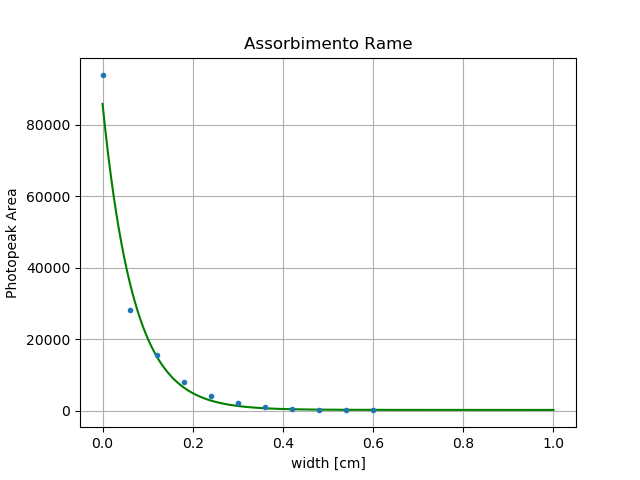
\includegraphics[width=1\textwidth]{assorbimento_rame}
        \caption{Fig. 24: Grafico dell'attenuazione dell'intensità della radiazione in funzione dello spessore di Rame, i punti sono fittati tramite una funzione esponenziale.}
        \label{fig:24}
\end{figure}

\section{Giunzione in polarità inversa}
In questa seconda parte abbiamo modificato le impostazioni della catena di acquisizione dati. Si inseriscono:
\begin{itemize}
\item Discriminatore: collegato in uscita all’amplificatore,
\item Contatore: calcolando l’integrale dei picchi rivelati, restituisce i conteggi totali.
\end{itemize}

Operiamo sulla tensione di soglia $V_{th}$ (in mV) del discriminatore e ne visualizziamo gli effetti su diversi segnali (test, sorgente). Il discriminatore rivela eventi solo al di sopra di $V_{th}$, pertanto ci aspettiamo che, all’aumentare della tensione di soglia, diminuiscano
i conteggi sul contatore. Con segnali test, quando la soglia è bassa, ci aspettiamo di trovare i conteggi a partire dalla frequenza del segnale in ingresso e dalla time unit del contatore Basandoci su ciò, valutiamo diverse configurazionidel sistema usando prima il segnale test e successivamente inserendo la sorgente di Americio.
Cerchiamo:
\begin{itemize}
\item il punto in cui il conteggio è $\simeq 0$ o comunque minimo,
\item il punto in cui il conteggio è al 50 %,
\item il punto in cui sono rivelati all’incirca tutti gli eventi aspettati
\end{itemize}

I valori così ottenuti possono essere fittati con una funzione di slope decrescente (\emph{sigmoide}):
\begin{equation}
f(x)= A_{2} + \frac{A_{1}-A_{2}}{1+e^{\frac{x-m}{s}}}
\end{equation}

dove m è il valore di ascissa ($V_{th}$) a cui si ha metà dei conteggi e s è la derivata della funzione in quel punto; $A_{1}$ è il massimo dei conteggi e $A_{2}$ il minimo. Valuteremo la pendenza della sigmoide per diversi condensatori. Dopodichè inseriremo la sorgente di Cadmio e valuteremo l’andamento dei conteggi al variare della tensione di soglia del discriminatore.\\ 
Il range di discriminazione è \textbf{50-250 mV}, per cui è ragionevole mandare segnali di circa e non oltre 200 mV. Questo, però, ci impedisce di analizzare con questo metodo l'Americio, in quanto non si ha una tensione di soglia sufficiente (più di 400 mV di $V_{th}$), quindi bisognerebbe cambiare amplificazione per poterlo vedere, ma stareremmo tutta la strumentazione.\\
Riprendiamo, quindi, il segnale simulato a 22.6 KeV osservandolo tramite l'oscilloscopio. Per farlo generiamo un segnale a \textbf{1.50 mV}, avendo un'attenuazione di \textbf{46 dB} (40 dB rotella + 6 dB pulsanti).\\ 
Viene quindi cambiato il setup \textbf{con il rivelatore in polarità inversa} e la tensione di svuotamento rimane quella trovata precedentemente (\textbf{12 V}).
Settiamo l'amplificazione per avere il segnale che vogliamo, quello ottenuto è di \textbf{180 mV} circa. \\
\subsection{Conteggi al variare della tensione di soglia.}
Vogliamo ricostruire la curva tensione-conteggi.\\
Mandiamo dall'amplificatore il segnale al discriminatore e osserviamo il segnale all'oscilloscopio, dal quale si notano 2 segnali separati: uno corrisponde al fronte di salita, l'altro a quello di discesa. Ci accorgiamo, quindi, che il discriminatore è troppo veloce e vi sono più conteggi di quelli effettivi. Per far sì che conti il giusto numero di input, abbiamo bisogno di allungare il tempo del segnale, portiamo allora il segnale simulato dal generatore al valore di \textbf{5 mV}. Tempo d'acquisizione: \textbf{10 s}.
Viene fatta una prima misura a vuoto, poi inseriamo le capacità studiate precedentemente (i cavetti LEMO) sul rivelatore e controlliamo i conteggi.

\begin{table}[H]
	
		\begin{tabular}{lcc}
			\hline
			\hline
			\textbf{$V_{th}$} [mV] & \textbf{Counts}  	\\
			\hline
			\hline
				      125.1 &  5122   	\\
				      138.9 &  5121     \\
				      142.8 &  5120	  \\
				      152.4 &  4846	 \\
				      156.0 &  4832	 \\
				      160.7 &  3271	 \\
				      166.3 &  2159	  \\
				      170.9 &  1546	 \\
				      174.6 &  1023	 \\
				      176.0 &  535	  \\
				      177.3 &  455  \\
				      178.4 &  377  \\
				      182.0 &  207  \\
				      191.8 &  206  \\
			\hline
			\hline
		\end{tabular}
		\linebreak
		\caption{\textit{Tabella 12: Dati a vuoto al variare della tensione di soglia.}}\label{tab:12} 
	\end{table}	

\begin{table}[H]
	
		\begin{tabular}{lcc}
			\hline
			\hline
			\textbf{$V_{th}$} [mV] & \textbf{Counts}  	\\
			\hline
			\hline
				      123.0 &  5122	 \\
				      141.0 &  5104	 \\
				      152.0 &  4916	 \\
				      163.7 &  3606	  \\
				      167.4 &  3020	 \\
				      173.9 &  1470	 \\
				      180.9 &  629	  \\
				      190.6 & 58  \\
				      195.4 &  13  \\
				      
			\hline
			\hline
		\end{tabular}
		\linebreak
		\caption{\textit{Tabella 13: Dati ottenuti con un capacità $C=27.1 pF$.}}\label{tab:13} 
	\end{table}	
	
	\begin{table}[H]
	
		\begin{tabular}{lcc}
			\hline
			\hline
			\textbf{$V_{th}$} [mV] & \textbf{Counts}  	\\
			\hline
			\hline
				      130.0 &  5122	 \\
				      142.0 &  5117 \\
				      143.4 &  5112	 \\
				      151.0 &  4967	  \\
				      158.5 &  4500	 \\
				      161.2 &  4064	 \\
					  163.5 & 3788		\\		      
				      167.4.9 &  2797	  \\
				      169.4 & 2059  \\
				      178.5 & 852  \\
				      180.4 & 149 \\
					  192.8 & 8 \\			
			\hline
			\hline
		\end{tabular}
		\linebreak
		\caption{\textit{Tabella 14: Dati ottenuti con un capacità $C=18.6 pF$.}}\label{tab:14} 
	\end{table}	
	
	\begin{table}[H]
	
		\begin{tabular}{lcc}
			\hline
			\hline
			\textbf{$V_{th}$} [mV] & \textbf{Counts}  	\\
			\hline
			\hline
				      125.2 &  5122	 \\
				      135.1 &  5122	 \\
					  142.2	&  5121	\\		      
				      150.2 &  5166	 \\
				      159.4 &  4446	  \\
				      164.0 &  3544	 \\
				      170.8 &  2497	 \\
					  175.2 &  1591		\\		      
				      179.1 &  586	  \\
				      185.3 & 258  \\
				      193.1 &  11  \\
				      
			\hline
			\hline
		\end{tabular}
		\linebreak
		\caption{\textit{Tabella 15: Dati ottenuti con un capacità $C=12.4 pF$.}}\label{tab:15} 
	\end{table}	
I dati raccolti ci consentono di fare un fit dei dati tramite una funzione sigmoide, da cui possiamo ricavare così i valori $A_{1}$, $A_{2}$, m ed s. In Fig. 21,22,23,24 presentiamo i fit e le relative funzioni ricavate.

\begin{figure}[H]
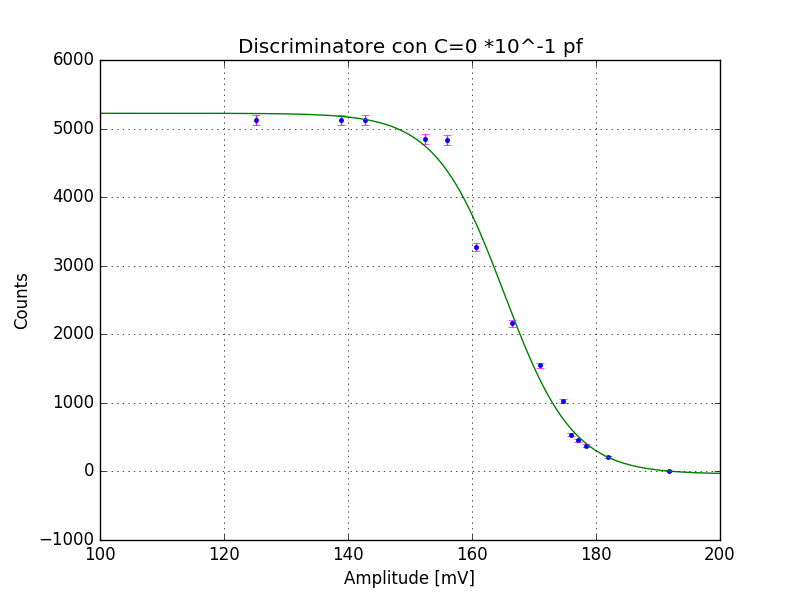
\includegraphics[width=1\textwidth]{discriminatore_0C}
        \caption{Fig. 25: Conteggi al variare della tensione di soglia, rilevatore senza capacità..}
        \label{fig:25}
\end{figure}
\begin{equation}
f(x)_{vuoto}= -61.40 + \frac{5115.21+61.40}{1+e^{\frac{x-173.02}{184.65}}}
\end{equation}

\begin{figure}[H]
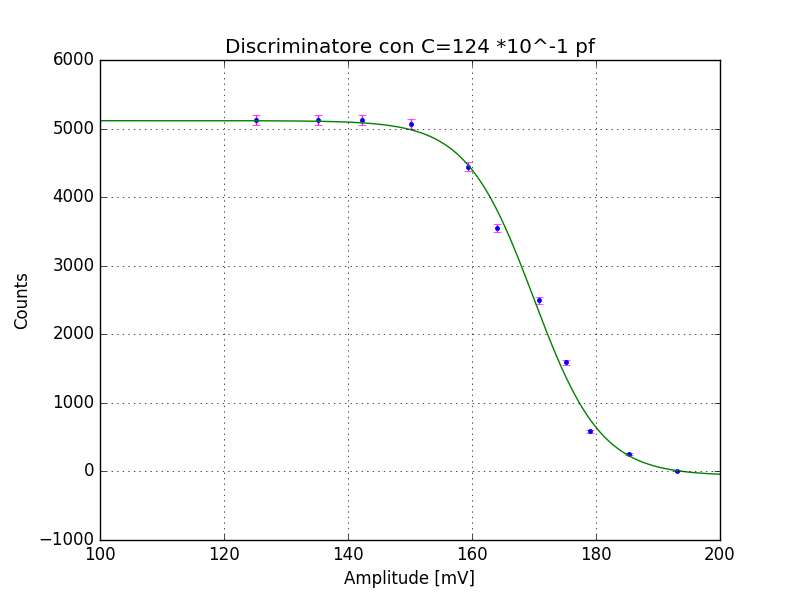
\includegraphics[width=1\textwidth]{discriminatore_124C}
        \caption{Fig. 26: Conteggi al variare della tensione di soglia, C=12.4 pF.}
        \label{fig:26}
\end{figure}
\begin{equation}
f(x)_{12.4 pF}= -47.35 + \frac{5172.25+47.35}{1+e^{\frac{x-177.43}{189.46}}}
\end{equation}

\begin{figure}[H]
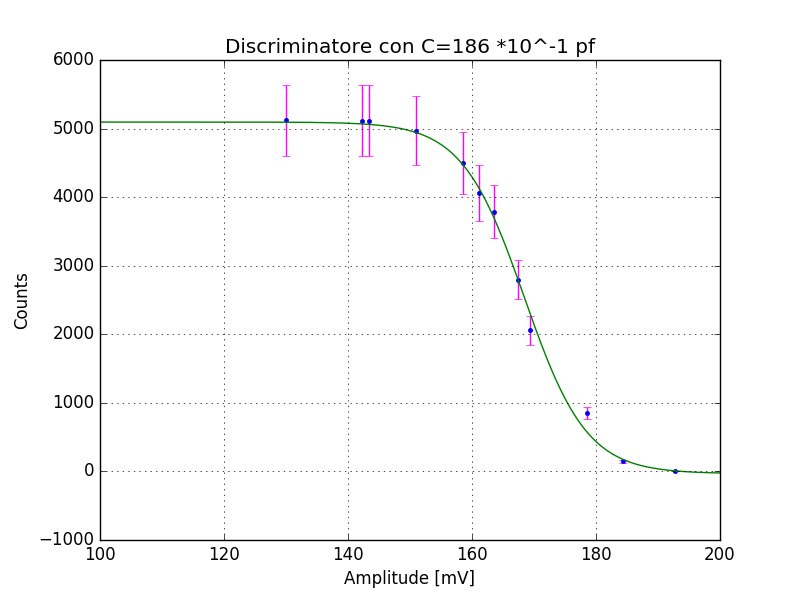
\includegraphics[width=1\textwidth]{discriminatore_186C}
        \caption{Fig. 27: Conteggi al variare della tensione di soglia, C=18.6 pF.}
        \label{fig:27}
\end{figure}
\begin{equation}
f(x)_{18.6 pF}= -12.20 + \frac{341.63+12.20}{1+e^{\frac{x-175.76}{190.51}}}
\end{equation}

\begin{figure}[H]
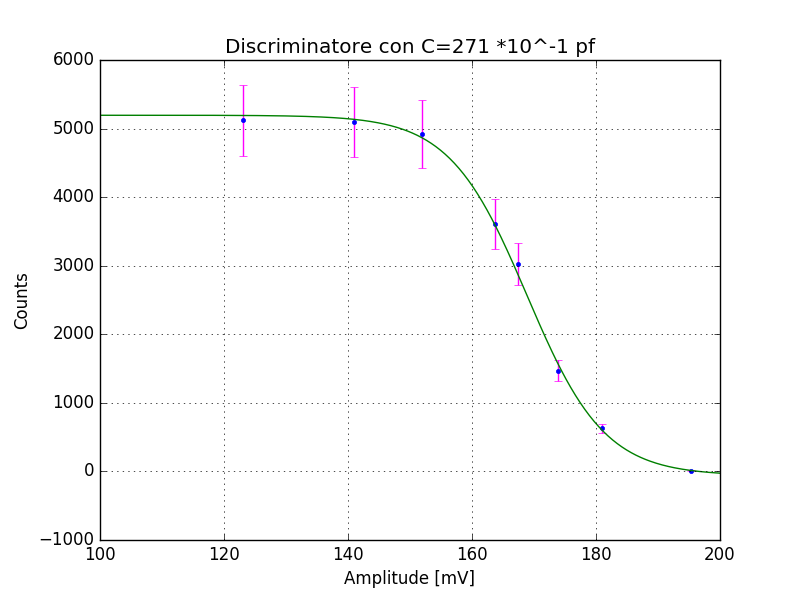
\includegraphics[width=1\textwidth]{discriminatore_271C}
        \caption{Fig. 28: Conteggi al variare della tensione di soglia, C=27.1 pF.}
        \label{fig:28}
\end{figure}
\begin{equation}
f(x)_{27.1}= -51.25 + \frac{5158+51.25}{1+e^{\frac{x-167.35}{3.23}}}
\end{equation}
\newpage


\begin{comment}
\subsection{Calibrazione con rilevatore}
Vogliamo ottenere una calibrazione del setup con delle sorgenti radioattive. Abbiamo sempre a disposizione la sorgente di Americio e Cadmio, la prima inutilizzabile a tale scopo perchè, come detto precedentemente, non abbiamo di 400 mV di soglia. Lavoriamo sempre alla tensione di 12V sul rivelatore, scegliamo come tempo di acquisizione \textbf{100 s}.\\

Facciamo anzitutto una misura senza sorgente per valutare il rumore del sistema, poi una tramite il segnale simulato a 22.6 KeV con il generatore d'onde, con ampiezza $\Delta V = 1.50 mV$ e 46dB di attenuazione.\\
\begin{table}[H]
	
		\begin{tabular}{lcc}
			\hline
			\hline
			\textbf{$\Delta V$} [mV] & \textbf{Counts}  	\\
			\hline
			\hline
				      133.6 &  50818	 \\
				      140.0 &  50658	 \\
					  150.3	&  45013	\\		      
				      156.1 &  40628	 \\
				      161.4 &  25507	  \\
				      166.2 &  21081	 \\
				      171.5 &  10344	 \\
					  181.3 &  1453		\\		      
				      195.6 &  10	  \\
				      
			\hline
			\hline
		\end{tabular}
		\linebreak
		\caption{\textit{Tabella 16: Dati acquisizione rumore.}}\label{tab:16} 
	\end{table}	

\textbf{QUI DEVE ESSERE INSERITA LA TABELLA DEI VALORI OTTENUTI CON IL SEGNALE TEST A 20 KEV.}

\begin{table}[H]
	
		\begin{tabular}{lcc}
			\hline
			\hline
			\textbf{$\Delta V$} [mV] & \textbf{Counts}  	\\
			\hline
			\hline
				      133.6 &  50818	 \\
				      140.0 &  50658	 \\
					  150.3	&  45013	\\		      
				      156.1 &  40628	 \\
				      161.4 &  25507	  \\
				      166.2 &  21081	 \\
				      171.5 &  10344	 \\
					  181.3 &  1453		\\		      
				      195.6 &  10	  \\
				      
			\hline
			\hline
		\end{tabular}
		\linebreak
		\caption{\textit{Tabella 17: Dati acquisizione del segnale simulato a 20 KeV. \textbf{I DATI SU QUESTA TABELLA NON SONO GIUSTI E VANNO TROVATI}}}\label{tab:17} 
	\end{table}	



Dopo aver mandato il segnale test, inseriamo la sorgente di Cadmio. La soglia è alta così che si possano contare i segnali della sorgente con il discriminatore. Scansioniamo quindi la zona del picco, verificando i conteggi per diversi valori della $V_{th}$.

\begin{table}[H]
	
		\begin{tabular}{lcc}
			\hline
			\hline
			\textbf{$\Delta V$} [mV] & \textbf{Counts}  	\\
			\hline
			\hline
				      88 &  379	 \\
				      108.9 &  351	 \\
					  113.5	&  329	\\		      
				      120.1 &  342	 \\
				      122.4 &  342	  \\
				      125.2 &  315	 \\
				      130.6 &  324	 \\
					  135.3 &  290		\\		      
				      140.6 &  283	  \\
				      145.1 &  245 \\
				      150.3 &  226 \\
				      159.2 &  150 \\
				      166.7 &  75 \\
				      172.3 &  24 \\
				      180   &  9 \\
				      
			\hline
			\hline
		\end{tabular}
		\linebreak
		\caption{\textit{Tabella 18: Conteggi al variare della tensione di soglia.}}\label{tab:18} 
	\end{table}	
Vogliamo un ulteriore picco per per poter avere almeno 3 punti per la calibrazione, per cui simuliamo un segnale a \textbf{30 KeV}.

	\textbf{QUI VANNO INSERITI I DATI DEL DISCRIMINATORE CON IL SEGNALE SIMULATO A 30 KEV, QUINDI IL GRAFICO PER IL FIT DELLA CALIBRAZIONE E L'ESPRESSIONE DELLA RETTA DI CALIBRAZIONE.}


\end{comment}
  


\end{document}
%%%%%%%%%%%%%%%%%%%%%%%%